% Chapter Template

\chapter{Puzzles} % Main chapter title

\label{sec:Puzzles} % Change X to a consecutive number; for referencing this chapter elsewhere, use \ref{ChapterX}
%----------------------------------------------------------------------------------------
%	SECTION 1
%----------------------------------------------------------------------------------------

\section{Sliding Puzzle}


%-----------------------------------
%	SUBSECTION 1.1
%-----------------------------------
\subsection{History - The 15 Puzzle}


The first puzzle I will focus on is the sliding puzzle (see \cite{SlidingPuzzleWiki}).The 15-puzzle seems to have been invented in the late 19th century by Noyes Chapman (see \cite{SlidingPuzzleWolfram}), who applied for a patent in 1980. In 1879, a couple of interesting notes (\cite{Johnson1879}), published in the American Journal of Mathematics proved that exactly half of the $16!$ possible ways of setting up the 16 tiles on the board lead to solvable puzzles. A more modern proof can be found in \cite{Archer1999}.
\\
\\
Since then, several variations of the 15-puzzle have become popular, such as the 24-puzzle. A rather contrived but interesting one is the coiled 15-puzzle (\cite{Coiled15Puzzle}), where the bottom-right and the top-left compartments are adjascent; the additional move that this allows renders all $16!$ configurations solvable. 



\begin{figure}[H]
\centering
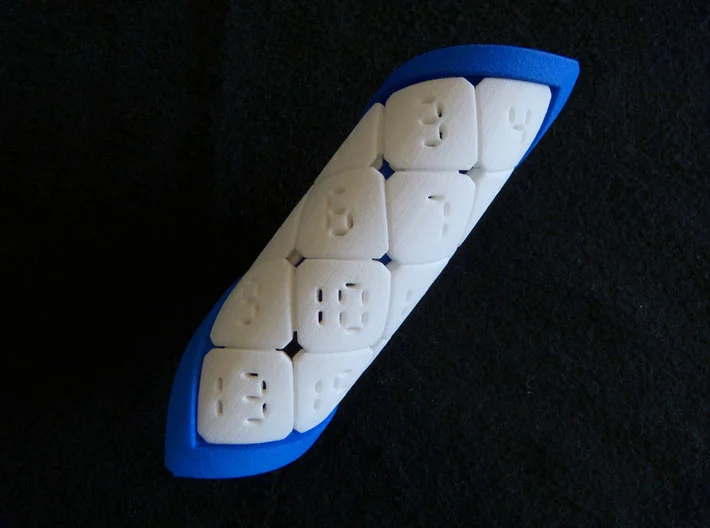
\includegraphics[scale=0.7]{./Figures/coiled15puzzle}
\decoRule
\caption[Coiled 15-puzzle]{Coiled 15-puzzle}
\label{fig:Coiled15Puzzle}
\end{figure}




It is rather easy to see why this is the case, let us discuss why: Given a configuration c of the tiles, let us define the permutation p(c) of this configuration according to the following schema: we enumerate the tiles row by row (top to bottom), left to right for odd rows and right to left for the even rows, ignoring the empty compartment. For instance, the following 15-puzzle c:

\begin{fifteen}
\setrow{4}{1,6,2,3}
\setrow{3}{5,10,7,4}
\setrow{2}{9,15,14,11}
\setrow{1}{13,12,,8}
\end{fifteen}
\\
\\
we have p(c) = (1, 6, 2, 3, 4, 7, 10, 5, 9, 15, 14, 11, 8, 12, 13).
\\
It is easy to see that the parity of p(c) cannot change by a legal move of the puzzle. Indeed, p(c) is clearly invariant by lateral move of a tile, so its parity is invariant too. A vertical move of a tile will displace a number in p(c) by an even number of positions right or left. For instance, moving tile 14 into the empty compartment above it results in a new configuration $c_{2}$:

\begin{fifteen}
\setrow{4}{1,6,2,3}
\setrow{3}{5,10,7,4}
\setrow{2}{9,15,,11}
\setrow{1}{13,12,14,8}
\end{fifteen}
\\
\\
with $p(c_{2})$ = (1, 6, 2, 3, 4, 7, 10, 5, 9, 15, 11, 8, 14, 12, 13), which is equivalent to moving 14 by 2 positions on the right. This obviously cannot change the parity since exactly 2 pairs of numbers are now in a different order, that is (14, 11) and (14, 8) now appear in the respective opposite orders as (11, 14) and (8, 14).
\\
\\
This is the crux of the proof of the well known necessary condition (even parity of p(c)) for a configuration c to be solvable (see part I of \cite{Johnson1879}).
\\
\\
In the case of the coiled puzzle, we can clearly solve all configurations of even parity, since all the legal moves of the normal puzzle are allowed. In addition, we can for instance transition between the following 2 configurations, which clearly have respectively even and odd parities:

\begin{fifteen}
\setrow{4}{1,2,3,4}
\setrow{3}{5,6,7,8}
\setrow{2}{9,10,11,12}
\setrow{1}{13,14,15,}
\end{fifteen}
%
\begin{fifteen}
\setrow{4}{,2,3,4}
\setrow{3}{5,6,7,8}
\setrow{2}{9,10,11,12}
\setrow{1}{13,14,15,1}
\end{fifteen}
\\
\\
Since it is possible to reach an odd parity configuration, and by symmetry arguments, we conclude we can solve all $16!$ configurations. 


%-----------------------------------
%	SUBSECTION 1.2
%-----------------------------------
\subsection{Search Space \& Solvability}

In this thesis, as well as in the code base (\cite{FB}) I have written to do this project, we will consider the general case of a board with n columns and m rows, where $(n, m) \in {\mathbb{N}^{+}}^{2}$, forming $n * m$ compartments. $n * m - 1$ tiles, numbered 1 to $n * m - 1$ are placed in all the compartments but one (which is left empty), and we can slide a tile directly adjascent to the empty compartment into it. Notice from a programming and mathematical analysis perspective, it is often easier to equivalently think of the empty compartment being moved (or swapped with) an adjacent tile. Starting from a given shuffling of the tiles on the board, our goal will be to execute moves until the tiles in ascending order: left to right, top to bottom (in the usual western reading order), the empty tile being at the very bottom right.
\\
\\
Note that the case where either n or m is 1 is uninteresting since we can only solve the puzzle if the tiles are in order to start with. For instance, in the (n, 1) case, we can only solve n of the $\frac{n!}{2}$ possible configurations. We will therefore only consider the case where both n and m are strictly greater than 1.




%-----------------------------------
%	SUBSECTION 1.3
%-----------------------------------
\subsection{Optimal Cost \& God's Number}

Let us fix n and m, integers strictly greater than 1 and call $\mathcal{C}_{(n, m)}$ the set of all $\frac{(n * m)!}{2}$ solvable configurations of the n by m sliding-puzzle. For any $c \in \mathcal{C}_{(n, m)}$ we define the optimal cost $\mathcal{O}(c)$ to be the minimum number of moves among all solutions for c. Finally we define $\mathcal{G}(n, m)$, God's number for the n by m puzzle as  $\mathcal{G}(n, m) = \max_{c \in \mathcal{C}_{(n, m)}} \mathcal{O}(c)$. Note that since $\frac{(n * m)!}{2}$ grows rather quickly with n and m, it is impossible to compute $\mathcal{G}$ except in rather trivial cases.
\\
\\
A favourite past time among computer scientists around the glove is therefore to search for more refined lower and upper bounds for $\mathcal{G}(n, m)$, for ever increasing values of n and m. For moderate n and m, we can actually solve optimally all possible configurations of the puzzle and compute exactly $\mathcal{G}(n, m)$  (using for instance $A^{*}$ and an admissible heuristic (recall \ref{GSH}, and we shall see modest examples of that in the results section later). For larger values of n and m (say 5 by 5), we do not know what the God number is. Usually, looking for a lower bound is done by \textit{guessing} hard configurations and computing their optimal path via an optimal search. Looking for upper bounds is done via smart decomposition of the puzzle into disjoint nested regions and for which we can compute an upper bound easily (either by combinatorial analysis or via exhaustive search). See for instance \cite{KarlemoOstergard} for an upper bound of 210 on $\mathcal{G}(5, 5)$.
\\
\\
A very poor lower bound can be always obtained by the following reasoning: each move can at best explore three new configurations (4 possible moves at best if the empty tile is not on a border of the board (less if it is): left, right, up, down but one of which is just going back to an already visited configuration). Therefore, after $p$ moves, we would span at best $\mathcal{S}(p) = \frac{3^{p+1} - 1}{2}$ configurations. A lower bound can thus be obtained for $\mathcal{G}(n, m)$ by computing the smallest integer $p$ for which $\mathcal{S}(p) \ge \frac{(n * m)!}{2}$


%-----------------------------------
%	SECTION 2
%-----------------------------------
\section{Rubiks' Cube}

blabla

